% Biên dịch bằng XeLaTeX (Overleaf: Menu -> Compiler -> XeLaTeX)
\documentclass[11pt]{article}

% Chế độ final (không ẩn danh) theo quy định đề bài
\usepackage[final]{acl}
\usepackage{microtype}
\usepackage{graphicx}
\usepackage{booktabs}
\usepackage{amsmath}
\usepackage{xcolor}

% Hỗ trợ tiếng Việt chuẩn cho XeLaTeX / LuaLaTeX
\usepackage[vietnamese]{babel}
\babelfont{rm}{TeX Gyre Termes} % Nếu báo thiếu font, đổi thành Liberation Serif

% Lệnh đánh dấu chỗ cần điền tiếp sau khi chạy xong các thí nghiệm GPU còn lại
\newcommand{\todo}[1]{\textcolor{red}{\textbf{[TODO: #1]}}}

\title{Phát hiện Biển báo Giao thông Việt Nam từ Ảnh Camera Hành trình:\\Phân tích Vật thể Nhỏ và So sánh Kiến trúc Một giai đoạn -- Hai giai đoạn}

\author{
  \textbf{Đỗ Hoàng Minh} (MSSV: \todo{MSSV1}) \quad
  \textbf{Thành viên 2} (MSSV: \todo{MSSV2}) \quad
  \textbf{Thành viên 3} (MSSV: \todo{MSSV3}) \\
  Nhóm 06 -- Học phần Học sâu (AIT3001) \\
  \texttt{https://github.com/dohoangminh-vn/AIT3001.Group6.traffic.sign.detection}
}

\begin{document}
\maketitle

% ====================================================================
\begin{abstract}
Phát hiện và phân loại biển báo giao thông từ camera hành trình (dashcam) là bài toán cốt lõi trong các hệ thống hỗ trợ lái xe tiên tiến (ADAS). Tuy nhiên, trong bối cảnh đường phố Việt Nam, bài toán đối mặt với ba thách thức nghiêm trọng: tỷ lệ biển báo kích thước nhỏ áp đảo, mất cân bằng lớp lớn và nền đô thị phức tạp chứa nhiều biển quảng cáo dễ gây nhầm lẫn. Trên bộ dữ liệu Zalo AI Challenge Traffic Sign (4.500 ảnh độ phân giải $1622\times 626$, 7 lớp), quá trình khảo sát dữ liệu của chúng tôi phát hiện hai vấn đề hệ thống quan trọng: (i) 10,13\% hộp nhãn gốc (1.114/11.000) bị gán trùng đè và (ii) toàn bộ ảnh chỉ đến từ 38 tuyến đường (\texttt{street\_id}), gây nguy cơ rò rỉ dữ liệu nếu chia ngẫu nhiên. Chúng tôi xây dựng quy trình làm sạch nhãn, chia tập theo nhóm \texttt{street\_id} (0\% rò rỉ), và đánh giá công bằng trên cùng bộ chấm \texttt{pycocotools} giữa hai họ kiến trúc tiêu biểu: Một giai đoạn (YOLOv8, \todo{YOLO26}) và Hai giai đoạn (Faster R-CNN tùy biến Small Anchors), kết hợp các kỹ thuật mở rộng cho vật thể nhỏ (tăng độ phân giải đầu vào, SAHI cắt lát) và xử lý mất cân bằng lớp. Kết quả baseline \texttt{YOLOv8s} ($640\times 640$) đạt \texttt{mAP@0.5} = 0,5564 và \texttt{mAP@0.5:0.95} = 0,3608, nhưng \texttt{AP\_small} chỉ đạt 0,2704 (so với \texttt{AP\_medium} = 0,6972), với 93,4\% lỗi bỏ sót rơi vào biển báo nhỏ. \todo{Cập nhật kết quả tốt nhất sau khi hoàn tất 1280, Faster R-CNN và SAHI.}
\end{abstract}

% ====================================================================
\section{Giới thiệu}
\label{sec:intro}

Hệ thống phát hiện biển báo giao thông tự động đóng vai trò quan trọng trong việc cảnh báo người lái và đảm bảo an toàn giao thông. Khác với các bộ dữ liệu phương Tây, ảnh chụp từ camera hành trình tại Việt Nam có góc rộng ($1622\times 626$ pixel), mật độ phương tiện cao, ánh sáng thay đổi mạnh và đặc biệt là nhiều biển quảng cáo có màu sắc đỏ--vàng--xanh tương đồng với biển báo cấm và hiệu lệnh.

\paragraph{Phát biểu bài toán.}
Đầu vào của hệ thống là một ảnh màu RGB $\mathbf{I} \in \mathbb{R}^{H \times W \times 3}$ chụp từ camera hành trình. Đầu ra là tập hợp các dự đoán $\{(b_i, c_i, s_i)\}_{i=1}^{N}$, trong đó $b_i = (x_i, y_i, w_i, h_i)$ là tọa độ bounding box, $c_i \in \{1,\dots,7\}$ là nhãn loại biển báo Việt Nam và $s_i \in [0, 1]$ là độ tin cậy.

\paragraph{Đóng góp chính.}
Các đóng góp chính của nhóm trong báo cáo này bao gồm:
\begin{enumerate}
  \item \textbf{Phân tích và làm sạch dữ liệu có hệ thống:} Phát hiện và loại bỏ 1.114 nhãn trùng lặp (10,13\%) trong bộ Zalo AI gốc; thiết kế chiến lược chia Train/Val/Test bằng \texttt{StratifiedGroupKFold} theo \texttt{street\_id} nhằm loại bỏ hoàn toàn rò rỉ dữ liệu.
  \item \textbf{Thiết lập benchmark công bằng giữa Một giai đoạn và Hai giai đoạn:} Đưa dự đoán của cả YOLOv8/YOLO26 và Faster R-CNN về cùng một bộ đánh giá chuẩn \texttt{pycocotools} (đã kiểm chứng \texttt{Oracle} = 1,0000).
  \item \textbf{Tối ưu chuyên biệt cho biển báo nhỏ (78,7\% dữ liệu):} Thực nghiệm kiểm soát các kỹ thuật tăng độ phân giải ($640 \rightarrow 1280$), tùy biến Small Anchors $(8\text{--}128)$ cho Faster R-CNN và suy luận cắt lát SAHI.
  \item \textbf{Phân tích lỗi chuyên sâu:} Chỉ rõ nguyên nhân định lượng (93,4\% lỗi bỏ sót là biển nhỏ) và định tính (báo động giả vào biển quảng cáo, mái cây xăng).
\end{enumerate}

% ====================================================================
\section{Các công trình liên quan}
\label{sec:related}

Các phương pháp phát hiện vật thể hiện đại bằng học sâu thường được chia thành hai nhánh chính:

\paragraph{Kiến trúc Hai giai đoạn (Two-Stage).}
\citet{ren2015faster} đề xuất Faster R-CNN kết hợp mạng đề xuất vùng (Region Proposal Network -- RPN) với đầu phân loại RoI để đạt độ chính xác cao. Để cải thiện phát hiện đa tỷ lệ, \citet{lin2017fpn} giới thiệu Feature Pyramid Network (FPN) kết hợp đặc trưng ngữ nghĩa sâu với bản đồ độ phân giải cao ở tầng nông.

\paragraph{Kiến trúc Một giai đoạn (One-Stage).}
Họ mô hình YOLO khởi đầu bởi \citet{redmon2016yolo} dự đoán trực tiếp tọa độ và nhãn trong một lần truyền thẳng, mang lại tốc độ thời gian thực. Phiên bản YOLOv8 \citep{jocher2023yolov8} chuyển sang thiết kế Anchor-Free kết hợp Distribution Focal Loss (DFL), giúp cân bằng tốt giữa độ chính xác và tốc độ suy luận.

\paragraph{Vật thể nhỏ và biển báo giao thông.}
Các bộ dữ liệu lớn như COCO \citep{lin2014coco} và TT100K \citep{zhu2016tt100k} cho thấy hiệu năng suy giảm mạnh ở nhóm vật thể nhỏ ($<32^2$ px). Để khắc phục mà không cần tăng kích thước mô hình, \citet{akyon2022sahi} đề xuất SAHI (Slicing Aided Hyper Inference) cắt ảnh độ phân giải cao thành các mảnh chồng lấp khi suy luận rồi gộp bằng NMS. Trên tập Zalo AI Traffic Sign \citep{zalo2020traffic}, việc kết hợp độ phân giải cao và xử lý mất cân bằng lớp là chìa khóa nâng cao điểm mAP.

% ====================================================================
\section{Phương pháp}
\label{sec:method}

\subsection{Làm sạch dữ liệu và chia tập chống rò rỉ}
Qua khảo sát trực quan (trích xuất từ \texttt{01\_eda.py} và kiểm chứng ngược nhãn YOLO), chúng tôi phát hiện 1.114/11.000 hộp nhãn (10,13\%) trên 558 ảnh bị gán trùng đè cùng lớp với $\text{IoU} > 0{,}85$ (ví dụ ảnh \texttt{10424.png} có 4 hộp trùng đè lệch nhau đúng 1 pixel). Nếu giữ nguyên, khi mô hình dùng NMS chỉ giữ lại 1 hộp dự đoán, các hộp nhãn trùng còn lại sẽ bị tính oan thành False Negative làm sai lệch Recall và mAP. Do đó, chúng tôi loại bỏ các nhãn trùng ($\text{IoU} > 0{,}85$, cùng lớp), giữ lại 9.886 nhãn sạch.

Bên cạnh đó, 4.500 ảnh huấn luyện chỉ thuộc 38 tuyến đường (\texttt{street\_id}), trong đó tuyến lớn nhất (\texttt{street\_id=28}) có 626 khung hình liên tiếp. Chúng tôi sử dụng \texttt{StratifiedGroupKFold} ($K=6$, phân tầng theo lớp hiếm nhất trong ảnh, gom nhóm theo \texttt{street\_id}) để chia Train/Val/Test theo tỷ lệ 69,7\% / 16,0\% / 14,3\% với \textbf{0 tuyến đường trùng lặp} giữa các tập.

\subsection{Mô hình Một giai đoạn (YOLOv8)}
Chúng tôi huấn luyện \texttt{YOLOv8s} với hàm mất mát tổng hợp:
\begin{equation}
  \mathcal{L}_{\text{YOLO}} = \lambda_{\text{box}}\mathcal{L}_{\text{CIoU}} + \lambda_{\text{cls}}\mathcal{L}_{\text{BCE}} + \lambda_{\text{dfl}}\mathcal{L}_{\text{DFL}}.
\end{equation}
Một điều chỉnh quan trọng theo đặc thù bài toán là \textbf{tắt hoàn toàn phép lật ngang} (\texttt{fliplr = 0.0}), bởi việc lật ngang sẽ làm đảo ngược ngữ nghĩa của biển \textit{Cấm rẽ trái/phải} và đảo ngược chữ số trên biển \textit{Giới hạn tốc độ}.

\subsection{Mô hình Hai giai đoạn (Faster R-CNN tùy biến)}
Chúng tôi xây dựng kiến trúc \texttt{Faster R-CNN ResNet50-FPN-v2} kết hợp ba cải tiến chuyên biệt cho biển báo nhỏ và mất cân bằng lớp:
\begin{equation}
  \mathcal{L}_{\text{FRCNN}} = \mathcal{L}_{\text{obj}} + \mathcal{L}_{\text{rpn\_reg}} + \mathcal{L}_{\text{CB-Focal}} + \mathcal{L}_{\text{GIoU+L1}}.
\end{equation}
\begin{enumerate}
  \item \textbf{Small Sign Anchors:} Thống kê 6.590 hộp nhãn sạch cho thấy 90\% biển báo có tỷ lệ $h/w \in [0{,}74; 1{,}28]$ (trung vị $0{,}96$). Chúng tôi thay anchor mặc định bằng kích thước $(8, 16, 32, 64, 128)$ cùng tỷ lệ khung hình $(0{,}75; 1{,}0; 1{,}30)$ trên 5 tầng FPN (giữ nguyên 3 anchor/vị trí để tương thích trọng số RPN pretrained) và giữ độ phân giải gốc $(626, 1622)$.
  \item \textbf{RoIAlign $14\times 14$ và Class-Balanced Focal Loss tự cài đặt:} Nâng lưới \texttt{MultiScaleRoIAlign} từ $7\times 7$ lên $14\times 14$ (kèm \texttt{AdaptiveAvgPool2d(7)} trước lớp FC pretrained) để bảo toàn chi tiết mũi tên/chữ số bên trong lòng biển báo. Đồng thời, chúng tôi tự cài đặt lớp \texttt{FocalRoIHeads} áp dụng \citep{lin2017focal,cui2019class}: $\mathcal{L}_{\text{CB-Focal}} = -\alpha_y(1-p_y)^\gamma \log p_y$ với $\alpha_c \propto \frac{1-\beta}{1-\beta^{N_c}}$ và GIoU Loss \citep{rezatofighi2019generalized} nhằm xử lý lệch lớp $5{,}5\times$ và giảm nhầm lẫn giữa các biển cùng viền tròn.
  \item \textbf{Smart 3-Tile $640\times 640$ và Copy-Paste lớp hiếm:} Do chiều cao ảnh gốc là $626 \le 640$ px, chỉ cần 3 lát cắt ngang tại $x \in \{0, 491, 982\}$ (chồng lấp $149$ px = $23{,}3\%$) kết hợp 1 ảnh toàn cảnh tạo thành 1 batch 4 ảnh duy nhất khi suy luận SAHI \citep{akyon2022sahi}, đồng thời giữ 15\% lát cắt nền làm \textit{hard negative} và dán tăng cường mẫu của 3 lớp hiếm lúc huấn luyện.
\end{enumerate}

\subsection{Phân tách phần tự cài đặt và mã nguồn sẵn có}
Để đảm bảo tính minh bạch theo yêu cầu học phần, Bảng~\ref{tab:transparency} ghi rõ các thành phần nhóm tự xây dựng và các thư viện mã nguồn mở được sử dụng.

\begin{table}[t]
\centering
\small
\begin{tabular}{@{}p{0.44\linewidth}p{0.50\linewidth}@{}}
\toprule
\textbf{Nhóm tự cài đặt / tùy biến} & \textbf{Thư viện / Pretrained} \\
\midrule
Lọc trùng 2 tầng, chia \texttt{street\_id} \& config (\texttt{data\_utils.py}) & Ultralytics YOLOv8/26 (trọng số COCO) \\
Dataset, Copy-Paste \& Tiling 3 lát (\texttt{tiling.py}, \texttt{frcnn\_dataset.py}) & \texttt{torchvision} ResNet50-FPN-v2 \\
\texttt{FocalRoIHeads} (CB-Focal + GIoU), Small Sign AR \& RoI $14\times 14$ (\texttt{frcnn\_model.py}) & \texttt{pycocotools} (lõi tính AP chuẩn COCO) \\
Batch-4 SAHI + WBF, Grad-CAM \& Video FPS (\texttt{04..07}) & \texttt{albumentations}, \texttt{scikit-learn}, \texttt{wandb} \\
Hệ thống chấm tách lỗi 4 nhóm (\texttt{coco\_eval.py}, \texttt{05\_evaluate.py}) & -- \\
\bottomrule
\end{tabular}
\caption{Phân tách rõ ràng giữa thành phần nhóm tự cài đặt và thư viện mã nguồn mở sử dụng.}
\label{tab:transparency}
\end{table}

% ====================================================================
\section{Thực nghiệm}
\label{sec:experiments}

\subsection{Dữ liệu và phân tích khám phá (EDA)}
Bộ dữ liệu gốc Zalo AI Traffic Sign \citep{zalo2020traffic} gồm 4.500 ảnh huấn luyện (tất cả có kích thước $1622\times 626$ px) và 586 ảnh kiểm thử công khai không nhãn. Như minh họa tại Hình~\ref{fig:eda}, dữ liệu có hai đặc điểm cực đoan: (1) \textbf{mất cân bằng lớp 5,5 lần} giữa lớp nhiều nhất (\textit{Nguy hiểm}: 3.049) và lớp hiếm nhất (\textit{Cấm rẽ}: 556); (2) \textbf{78,7\%} nhãn là vật thể nhỏ ($<32^2$ px), trung vị chỉ $17\times 16$ px và nhỏ nhất $2\times 2$ px. Thống kê tập chia sau làm sạch được trình bày ở Bảng~\ref{tab:split}.

\begin{figure*}[t]
  \centering
  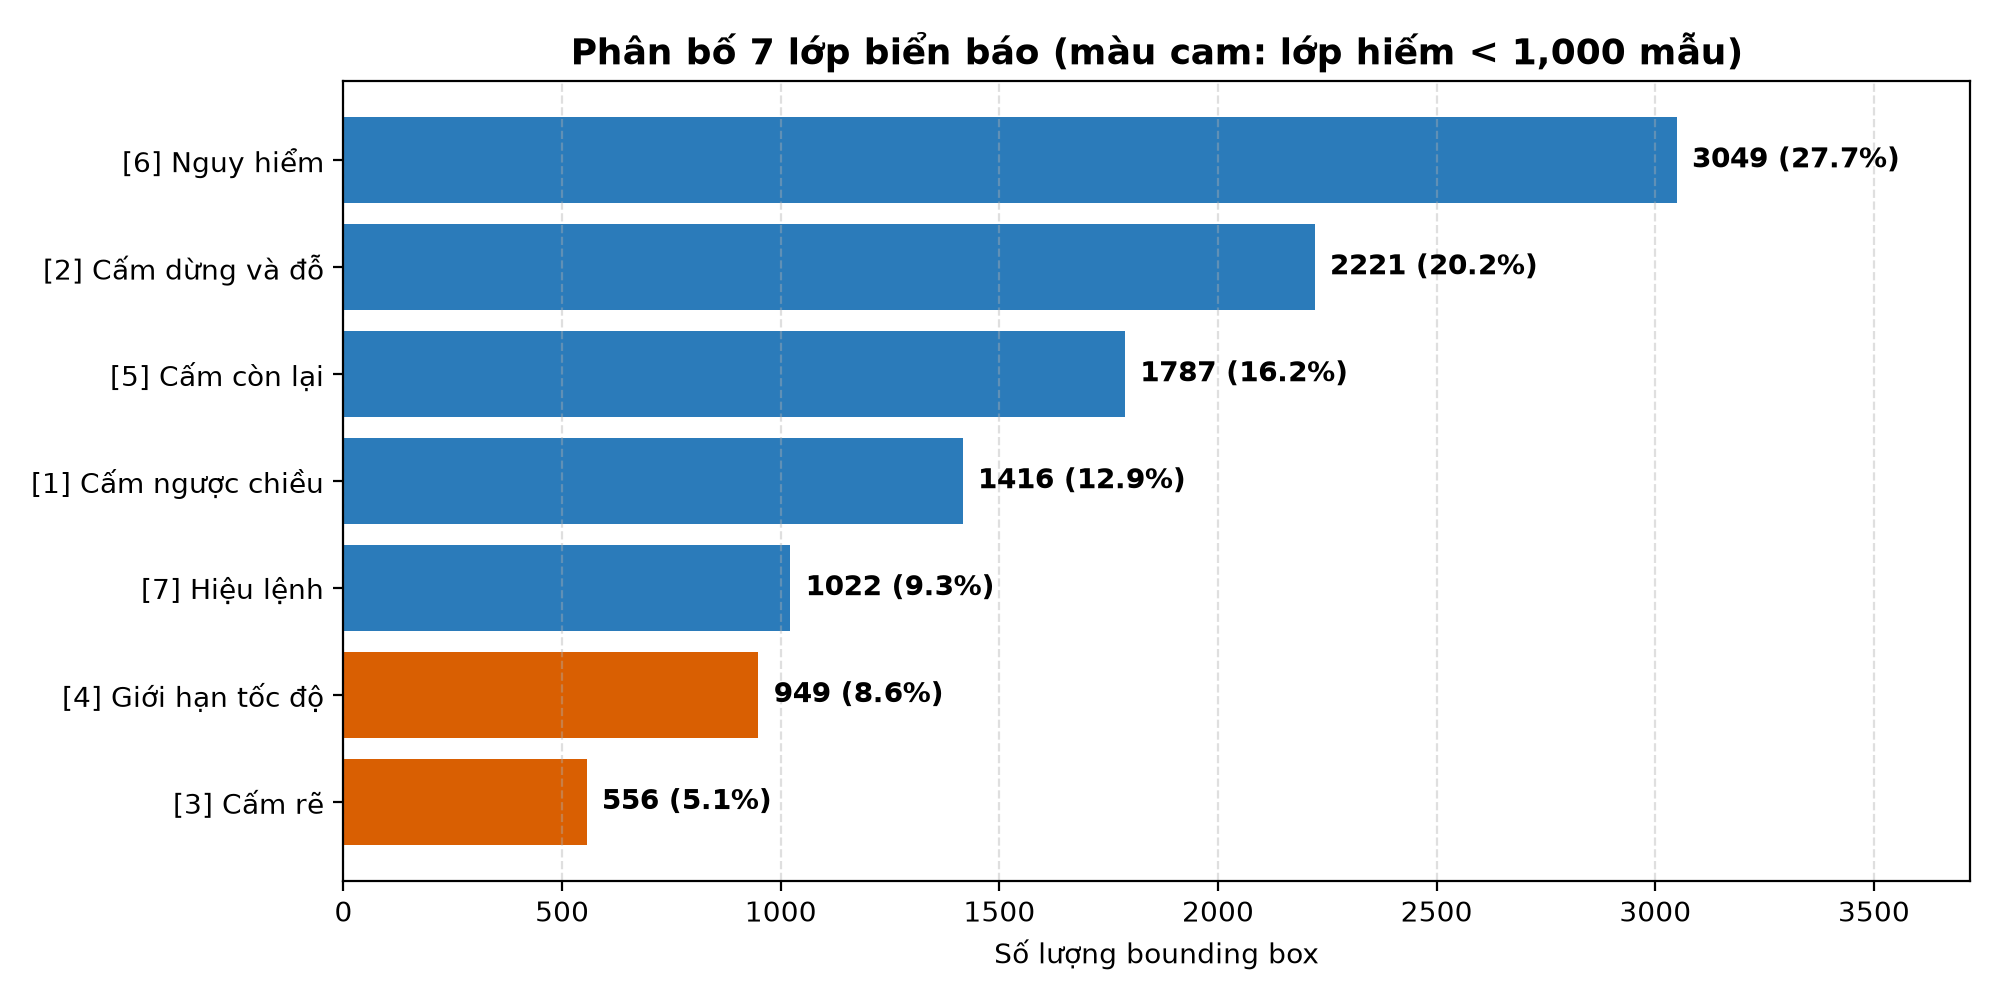
\includegraphics[width=0.49\textwidth]{figures/01_class_distribution.png}
  \hfill
  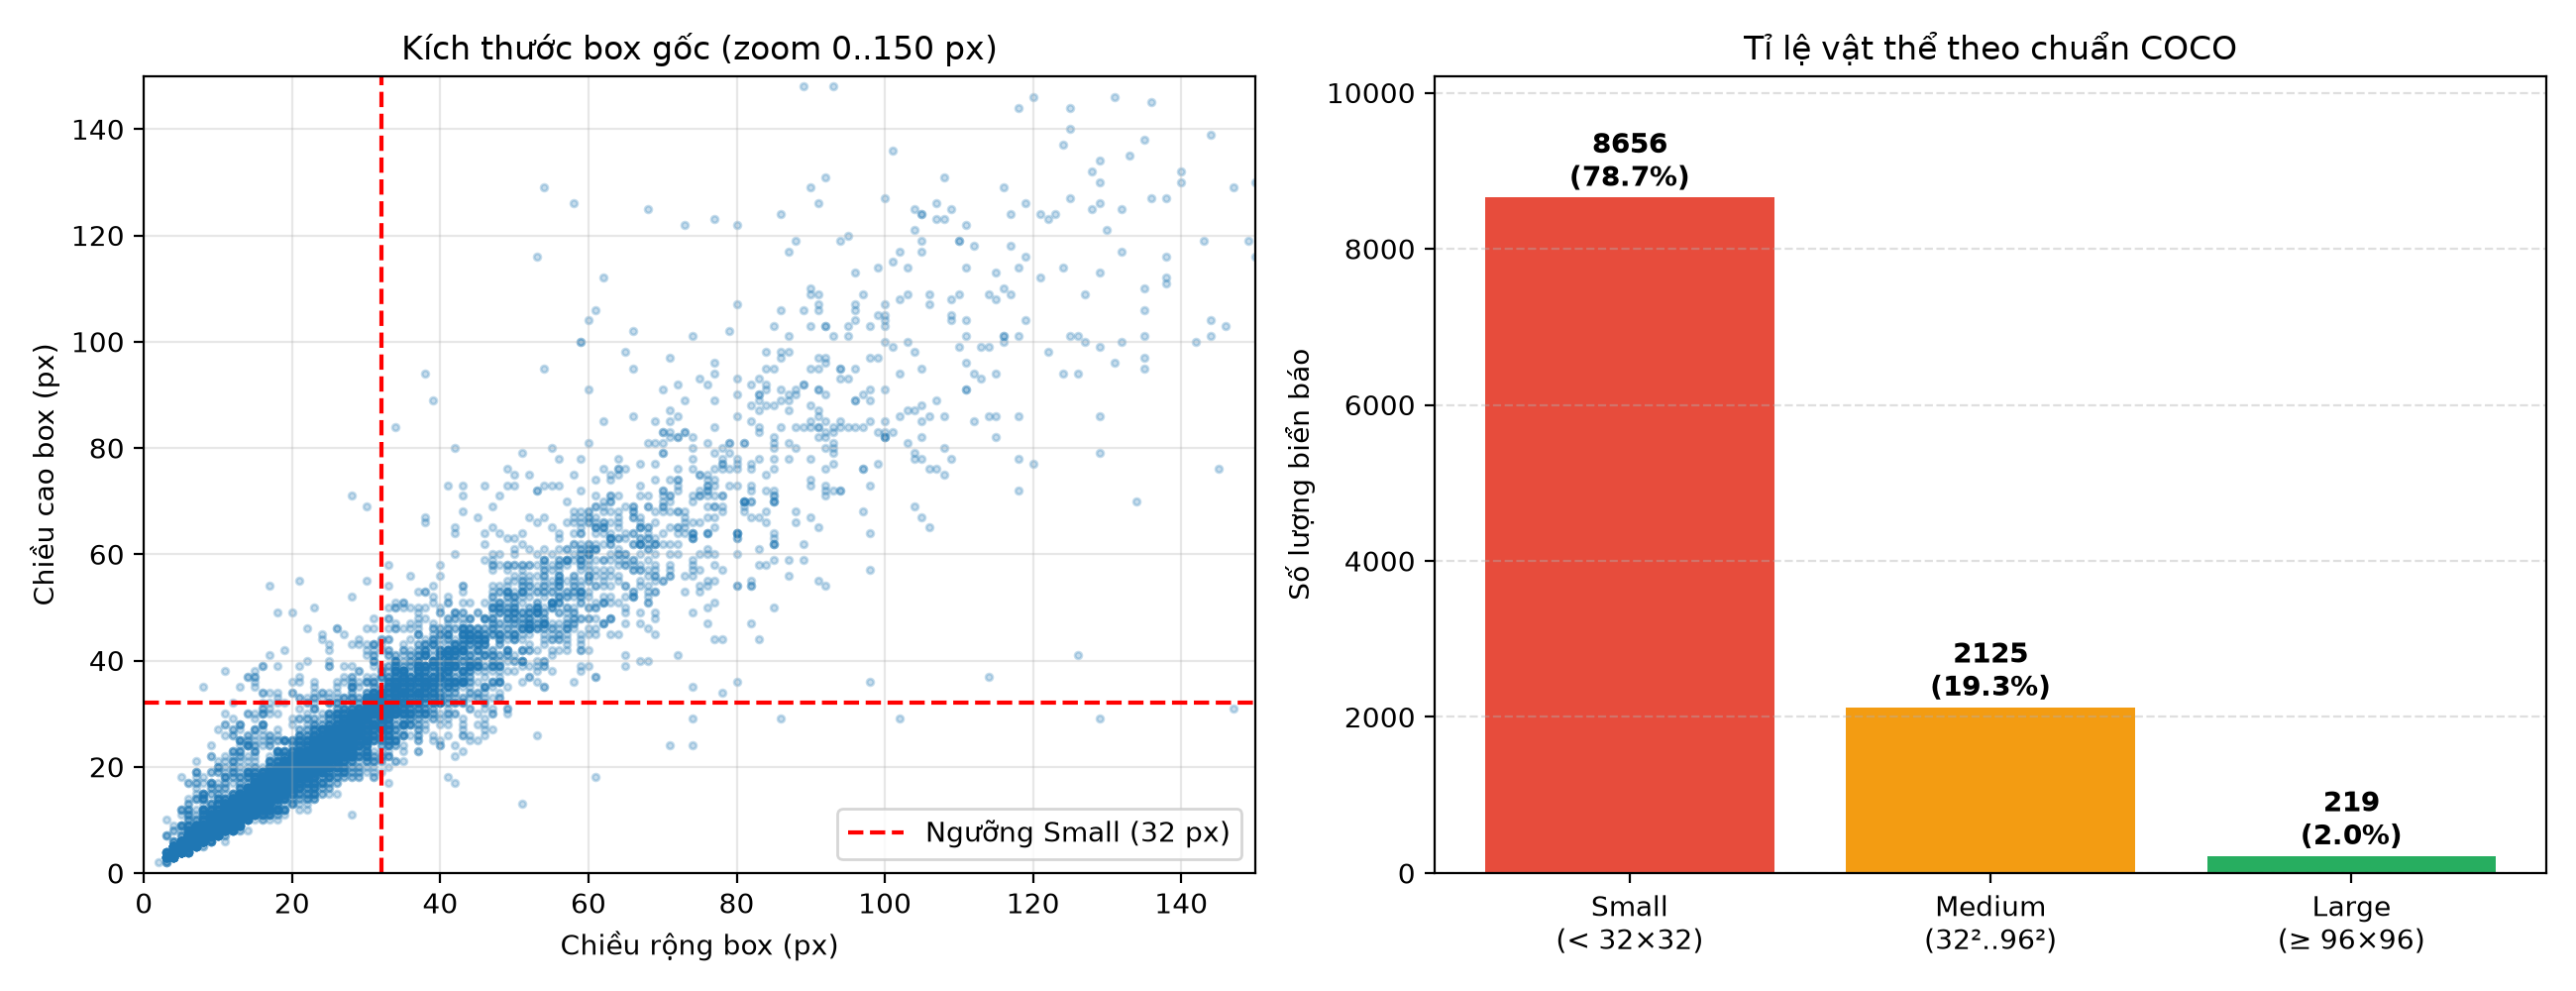
\includegraphics[width=0.49\textwidth]{figures/02_bbox_scale_analysis.png}
  \caption{Khám phá dữ liệu Zalo AI gốc: (trái) mất cân bằng giữa 7 lớp biển báo lên tới 5,5 lần; (phải) phân bố kích thước hộp nhãn với 78,7\% là vật thể nhỏ theo chuẩn COCO ($<32\times 32$ px).}
  \label{fig:eda}
\end{figure*}

\begin{table}[t]
\centering
\small
\begin{tabular}{@{}lrrrrr@{}}
\toprule
\textbf{Tập} & \textbf{Ảnh} & \textbf{Tỷ lệ} & \textbf{Streets} & \textbf{Box sạch} & \textbf{Lớp 3} \\
\midrule
Train & 3.135 & 69,7\% & 26 & 6.590 & 322 \\
Val   & 722   & 16,0\% & 6  & 1.733 & 89  \\
Test  & 643   & 14,3\% & 6  & 1.563 & 102 \\
\midrule
\textbf{Tổng} & \textbf{4.500} & \textbf{100\%} & \textbf{38} & \textbf{9.886} & \textbf{513} \\
\bottomrule
\end{tabular}
\caption{Thống kê chia dữ liệu sau lọc 1.114 nhãn trùng lặp. Không có \texttt{street\_id} nào trùng giữa ba tập.}
\label{tab:split}
\end{table}

\subsection{Thiết lập huấn luyện và chỉ số đánh giá}
Tất cả các mô hình được huấn luyện trên Kaggle GPU NVIDIA Tesla T4 (16 GB VRAM) với \texttt{seed = 42}. Để đảm bảo so sánh công bằng tuyệt đối giữa YOLO và Faster R-CNN, toàn bộ dự đoán được xuất ra cùng định dạng COCO JSON (ngưỡng tự tin \texttt{conf = 0.001}) và chấm bằng \texttt{pycocotools} trên các chỉ số: \texttt{mAP@0.5}, \texttt{mAP@0.5:0.95}, \texttt{AP\_small}, \texttt{AP\_medium}, \texttt{AP\_large} và tốc độ suy luận (FPS). Kiểm chứng \texttt{Oracle} đạt chính xác 1,0000 trên mọi chỉ số.

\subsection{Kết quả chính}
Bảng~\ref{tab:main_results} tổng hợp kết quả thực nghiệm trên tập Validation (722 ảnh, 1.733 biển báo sạch, trong đó 1.393 là biển báo nhỏ).

\begin{table*}[t]
\centering
\small
\begin{tabular}{@{}lcccccc@{}}
\toprule
\textbf{Mô hình / Cấu hình} & \textbf{mAP@0.5} & \textbf{mAP@0.5:0.95} & \textbf{AP\_small} & \textbf{AP\_medium} & \textbf{AP\_large} & \textbf{FPS} \\
\midrule
YOLOv8s ($640\times 640$, baseline) & 0,5564 & 0,3608 & 0,2704 & 0,6972 & 0,6161 & \todo{FPS} \\
YOLOv8s ($1280\times 1280$) & \todo{--} & \todo{--} & \todo{--} & \todo{--} & \todo{--} & \todo{--} \\
YOLO26s ($1280\times 1280$) & \todo{--} & \todo{--} & \todo{--} & \todo{--} & \todo{--} & \todo{--} \\
F0: Faster R-CNN (Default Anchors) & \todo{--} & \todo{--} & \todo{--} & \todo{--} & \todo{--} & \todo{--} \\
F1: + Small Sign Anchors $(8\text{--}128, \text{AR } 0{,}75\text{--}1{,}3)$ & \todo{--} & \todo{--} & \todo{--} & \todo{--} & \todo{--} & \todo{--} \\
F2: + Warmup \& \texttt{ReduceLROnPlateau} & \todo{--} & \todo{--} & \todo{--} & \todo{--} & \todo{--} & \todo{--} \\
F3: + CB-Focal + GIoU + RoI $14\times 14$ & \todo{--} & \todo{--} & \todo{--} & \todo{--} & \todo{--} & \todo{--} \\
F4: F3 + Batch-4 SAHI ($640\times 640$) & \todo{--} & \todo{--} & \todo{--} & \todo{--} & \todo{--} & \todo{--} \\
F5: Tiled $640$ (Copy-Paste + SAHI) & \todo{--} & \todo{--} & \todo{--} & \todo{--} & \todo{--} & \todo{--} \\
\bottomrule
\end{tabular}
\caption{So sánh hiệu năng chuẩn \texttt{pycocotools} trên tập Validation (722 ảnh sạch, không rò rỉ tuyến đường).}
\label{tab:main_results}
\end{table*}

% ====================================================================
\section{Phân tích}
\label{sec:analysis}

\subsection{Phân tích hiệu năng trên biển báo nhỏ}
Kết quả từ baseline \texttt{YOLOv8s-640} xác nhận mạnh mẽ giả thuyết từ bước EDA: trong khi mô hình đạt \texttt{AP\_medium} = 0,6972 và \texttt{AP\_large} = 0,6161, chỉ số \texttt{AP\_small} sụt giảm tới 42,7 điểm phần trăm xuống còn \textbf{0,2704}. Tại ngưỡng \texttt{conf = 0.25}, mô hình đạt 917 dự đoán đúng (TP), 255 báo động giả (FP) và bỏ sót 741 biển báo (FN) — trong đó có tới \textbf{692/741 (93,4\%)} là biển báo nhỏ. Nguyên nhân vật lý là ảnh gốc rộng 1622 px khi thu nhỏ về 640 px (hệ số 2,53$\times$) khiến biển báo trung vị $17\times 16$ px chỉ còn $\approx 6{,}7\times 6{,}3$ px, gần như bị triệt tiêu qua các tầng downsampling stride 8/16/32.

\subsection{Nghiên cứu cắt bỏ (Ablation Study)}
\todo{Bổ sung phân tích mức tăng $\Delta\text{AP\_small}$ khi tăng $640\rightarrow 1280$, đổi Small Anchors trên Faster R-CNN, bật SAHI cắt lát, và Copy-Paste cho lớp hiếm Cấm rẽ.}

\subsection{Phân tích lỗi định tính}
Kiểm tra trực quan các mẫu có nhiều lỗi nhất (như ảnh \texttt{4518.png} và \texttt{7124.png}) cho thấy ba nguồn lỗi điển hình:
\begin{itemize}
  \item \textbf{Bỏ sót biển báo ở chân trời (FN):} Các biển báo ở xa ($<15$ px) trên giàn treo hoặc lề đường bị mờ, lẫn vào tán cây.
  \item \textbf{Báo động giả vào nền đô thị Việt Nam (FP):} Mô hình dễ nhận nhầm các biển quảng cáo nền đỏ--vàng và logo mái cây xăng (ví dụ logo PV OIL trên ảnh \texttt{7124.png}) thành biển báo cấm do tương đồng mạnh về màu sắc và hình khối.
  \item \textbf{Nhầm lẫn giữa các biển cùng nhóm màu:} Các biển tròn viền đỏ (\textit{Cấm dừng đỗ}, \textit{Cấm rẽ}, \textit{Cấm còn lại}) khó phân biệt chi tiết bên trong khi kích thước nhỏ.
\end{itemize}
\todo{Chèn Hình 2: Ảnh phân tích lỗi \texttt{yolov8s\_640\_errors.png} và ảnh so sánh Trước/Sau SAHI.}

% ====================================================================
\section{Kết luận}
\label{sec:conclusion}
Chúng tôi đã xây dựng một quy trình hoàn chỉnh, minh bạch và chống rò rỉ dữ liệu cho bài toán phát hiện biển báo giao thông Việt Nam. Thực nghiệm chứng minh rằng việc làm sạch 10,13\% nhãn trùng lặp, chia tập theo tuyến đường và tối ưu chuyên biệt cho 78,7\% biển báo nhỏ là yếu tố quyết định chất lượng hệ thống. \todo{Hoàn thiện kết luận tổng hợp sau khi có đủ kết quả Faster R-CNN, 1280 và SAHI.}

% ====================================================================
% CÁC MỤC SAU ĐÂY KHÔNG TÍNH VÀO GIỚI HẠN 8 TRANG (BẮT BUỘC!)
% ====================================================================
\section*{Hạn chế (Limitations)}
Nghiên cứu của chúng tôi còn một số giới hạn cần lưu ý:
\begin{enumerate}
  \item \textbf{Giới hạn vật lý của nhãn gốc:} Bộ dữ liệu Zalo AI chứa các biển báo cực nhỏ tới $2\times 2$ px hoặc $4\times 4$ px (ví dụ lớp \textit{Hiệu lệnh}), nơi thông tin hình ảnh không đủ để phân biệt ngay cả bằng mắt người.
  \item \textbf{Độ đa dạng môi trường:} 4.500 ảnh chỉ thu thập trên 38 tuyến đường (chủ yếu ban ngày, trời khô), chưa đánh giá độ bền vững trong điều kiện ban đêm, mưa lớn hoặc chói đèn pha.
  \item \textbf{Xử lý từng khung hình độc lập:} Hệ thống hiện suy luận từng ảnh tĩnh, chưa khai thác thông tin theo dõi theo thời gian (object tracking) giữa các khung hình video liên tiếp.
  \item \textbf{Đánh đổi tốc độ khi cắt lát:} SAHI cải thiện \texttt{AP\_small} nhưng làm tăng độ trễ suy luận gấp nhiều lần so với suy luận đơn khung hình.
\end{enumerate}

\section*{Đóng góp của thành viên}
\begin{itemize}
  \item \textbf{Đỗ Hoàng Minh} (\todo{XX\%}): Khảo sát EDA, phát hiện và xử lý nhãn trùng lặp, thiết kế bộ chia chống rò rỉ theo \texttt{street\_id}, xây dựng pipeline đánh giá chuẩn \texttt{pycocotools}, huấn luyện baseline YOLOv8 và Faster R-CNN.
  \item \textbf{Thành viên 2} (\todo{XX\%}): \todo{Ghi rõ nhiệm vụ thực tế (vd: tiling, scheduler, W\&B, thí nghiệm mở rộng).}
  \item \textbf{Thành viên 3} (\todo{XX\%}): \todo{Ghi rõ nhiệm vụ thực tế (vd: phân tích lỗi, demo video, slide và báo cáo).}
\end{itemize}

\section*{Khai báo sử dụng công cụ AI}
Trong quá trình thực hiện bài tập lớn, nhóm có sử dụng công cụ trợ lý AI để hỗ trợ: (1) gợi ý cấu trúc tổ chức mã nguồn và khung LaTeX ACL, (2) gỡ lỗi kỹ thuật môi trường (lỗi bảng mã UTF-8 trên Windows với \texttt{pycocotools}, cấu hình XeLaTeX tiếng Việt), và (3) rà soát diễn đạt báo cáo. Toàn bộ quá trình chạy thực nghiệm, kiểm chứng dữ liệu, huấn luyện mô hình, kiểm thử đơn vị (\texttt{pytest}) và phân tích kết quả đều do các thành viên trực tiếp thực hiện và chịu trách nhiệm.

\bibliography{custom}

\appendix
\section{Phụ lục: Phân bố tuyến đường và mẫu biển báo}
\label{sec:appendix}
Hình~\ref{fig:appendix_streets} minh họa sự phân bố không đều của 4.500 khung hình trên 38 tuyến đường (\texttt{street\_id}) cùng 6 mẫu biển báo phóng to từ cực nhỏ ($4\times 4$ px) tới lớn ($163\times 111$ px).

\begin{figure*}[t]
  \centering
  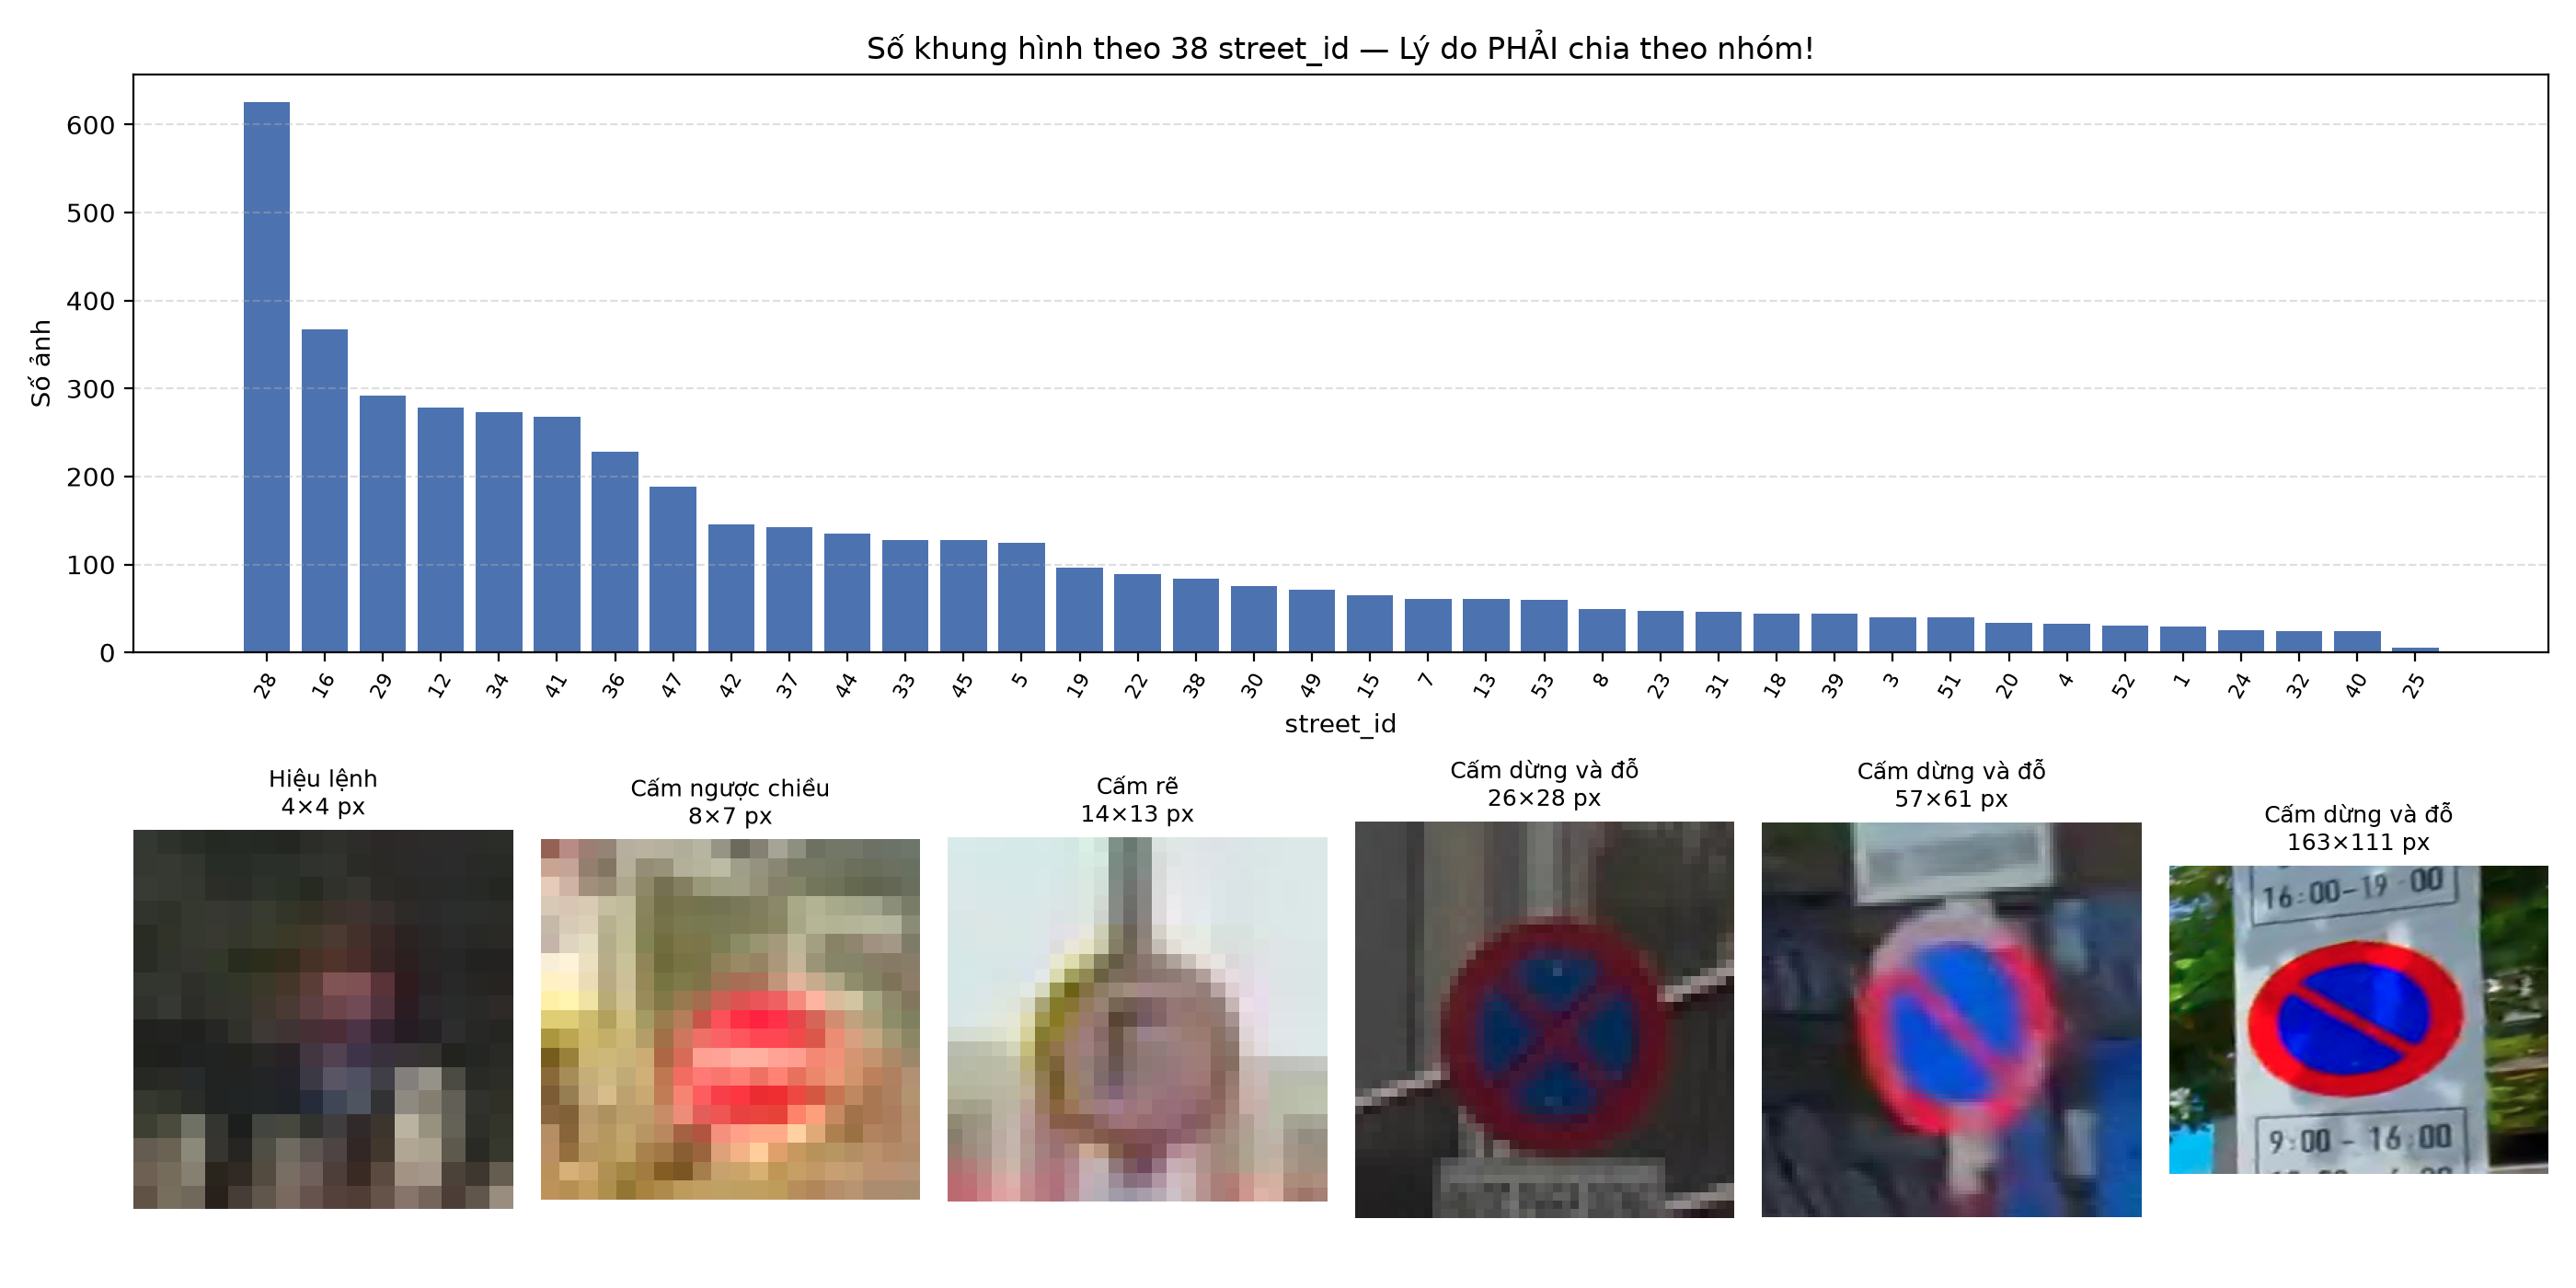
\includegraphics[width=0.95\textwidth]{figures/03_street_and_samples.png}
  \caption{Số lượng khung hình theo từng \texttt{street\_id} (trên) và 6 mẫu biển báo phóng to ở các kích thước khác nhau (dưới).}
  \label{fig:appendix_streets}
\end{figure*}

\end{document}